\section{Unit-tests}
At Unitteste er at teste enkelte moduler i koden. Vi tester vores kode for at fange eventuelle bugs og mangler på et tidligt stadie. Når man skriver sine tests, tvinges man samtidig til at tænke mere over det stykke kode man har skrevet.

\subsection{Hvordan Unittester vi?}
Vi bruger testframeworket NUnit. NUnit giver bla. mulighed for:
\begin{itemize}
	\item Detaljerede fejlrapporter - Beskriver hvorfor en test fejler.
	\item Setup og teardown, se figur \todo{indsæt eksempel på teardown og setup i NUnit}.
	\item At nemt indsætte nye tests i systemet.
\end{itemize}

Der er nogle konventioner man følger når man navngiver sine testmetoder.

\begin{lstlisting}
public void NameofUUT_NameOfMethodBeingTested_ExpectedOutcome()
\end{lstlisting}

Når der skrives en Unittest, følger man typisk de tre A'er.

\begin{itemize}
	\item Arrange - Opsætning af UUT. Ex sættes stubbe til at returnere det vi ønsker (udføres i Setup)
	\item Act - Stimuler UUT til at gøre det vi ønsker (udføres i testmetoden).
	\item Assert - Assertion på om vi får det forventede resultat (udføres i testmetoden).
\end{itemize}

\begin{figure}
\centering
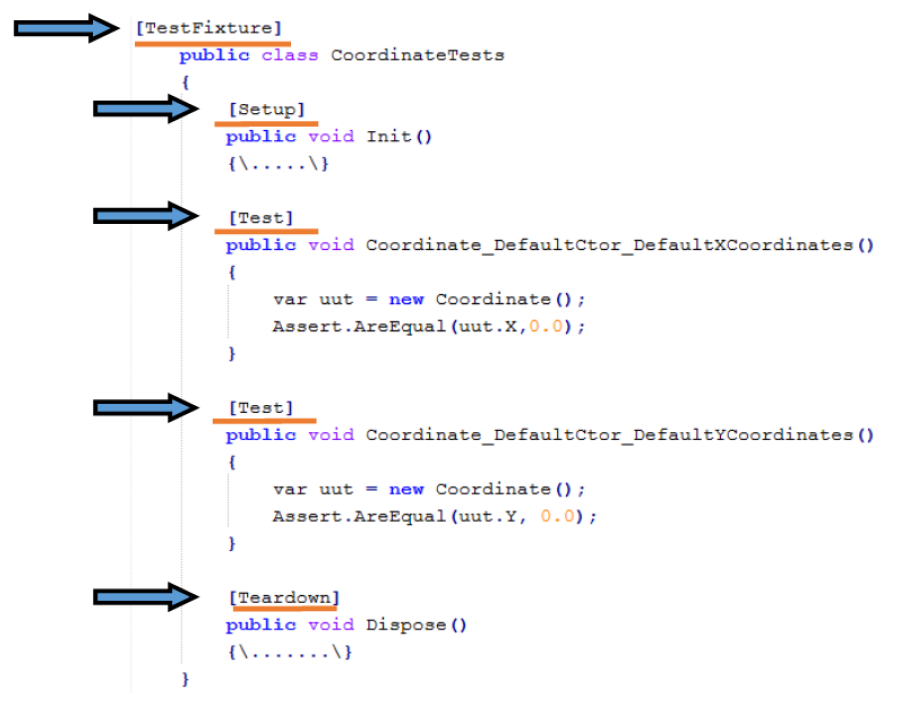
\includegraphics[width=0.7\linewidth]{figs/testFixture.PNG}
\caption{Syntaks for unittesting i NUnit}
\label{fig:testFixture}
\end{figure}
